\documentclass{assignment}
\ProjectInfos{研究型物理实验}{PHYS1703}{2020-2021学年第一学期}{Note-1-铷原子光谱简析}{2020. 09. 16(周三)}{陈稼霖}{45875852}
\begin{document}
\section*{要求}
\begin{itemize}
    \item[(1)] Rb超精细结构能量,以$e$V和GHz为单位;
    \item[(2)] 求$50^{\circ}$C下Rb原子的多普勒展宽;
    \item[(3)] 将(2)中的结果与P$_{3/2}$超精细结构的能量进行比较.
\end{itemize}
下面将在对铷原子光谱的简要分析的过程中顺带完成上述的要求.

\section{铷原子超精细结构能量}
铷原子存在两种同位素——\ce{^{85}Rb}和\ce{^{87}Rb},其丰度分别为$72\%$和$28\%$. 两种同位素原子的S轨道和P轨道能级如图\ref{Rb-energy-level}所示:由于自旋轨道耦合,P能级分裂为P$_{1/2}$和P$_{3/2}$,为精细结构,能量劈裂差值量级为$10^0 e$V;由于电子自旋磁矩和核磁矩之间的耦合,S$_{1/2}$、P$_{1/2}$、P$_{3/2}$又各自有进一步的劈裂,为超精细结构.
\begin{figure}[h]
    \centering
    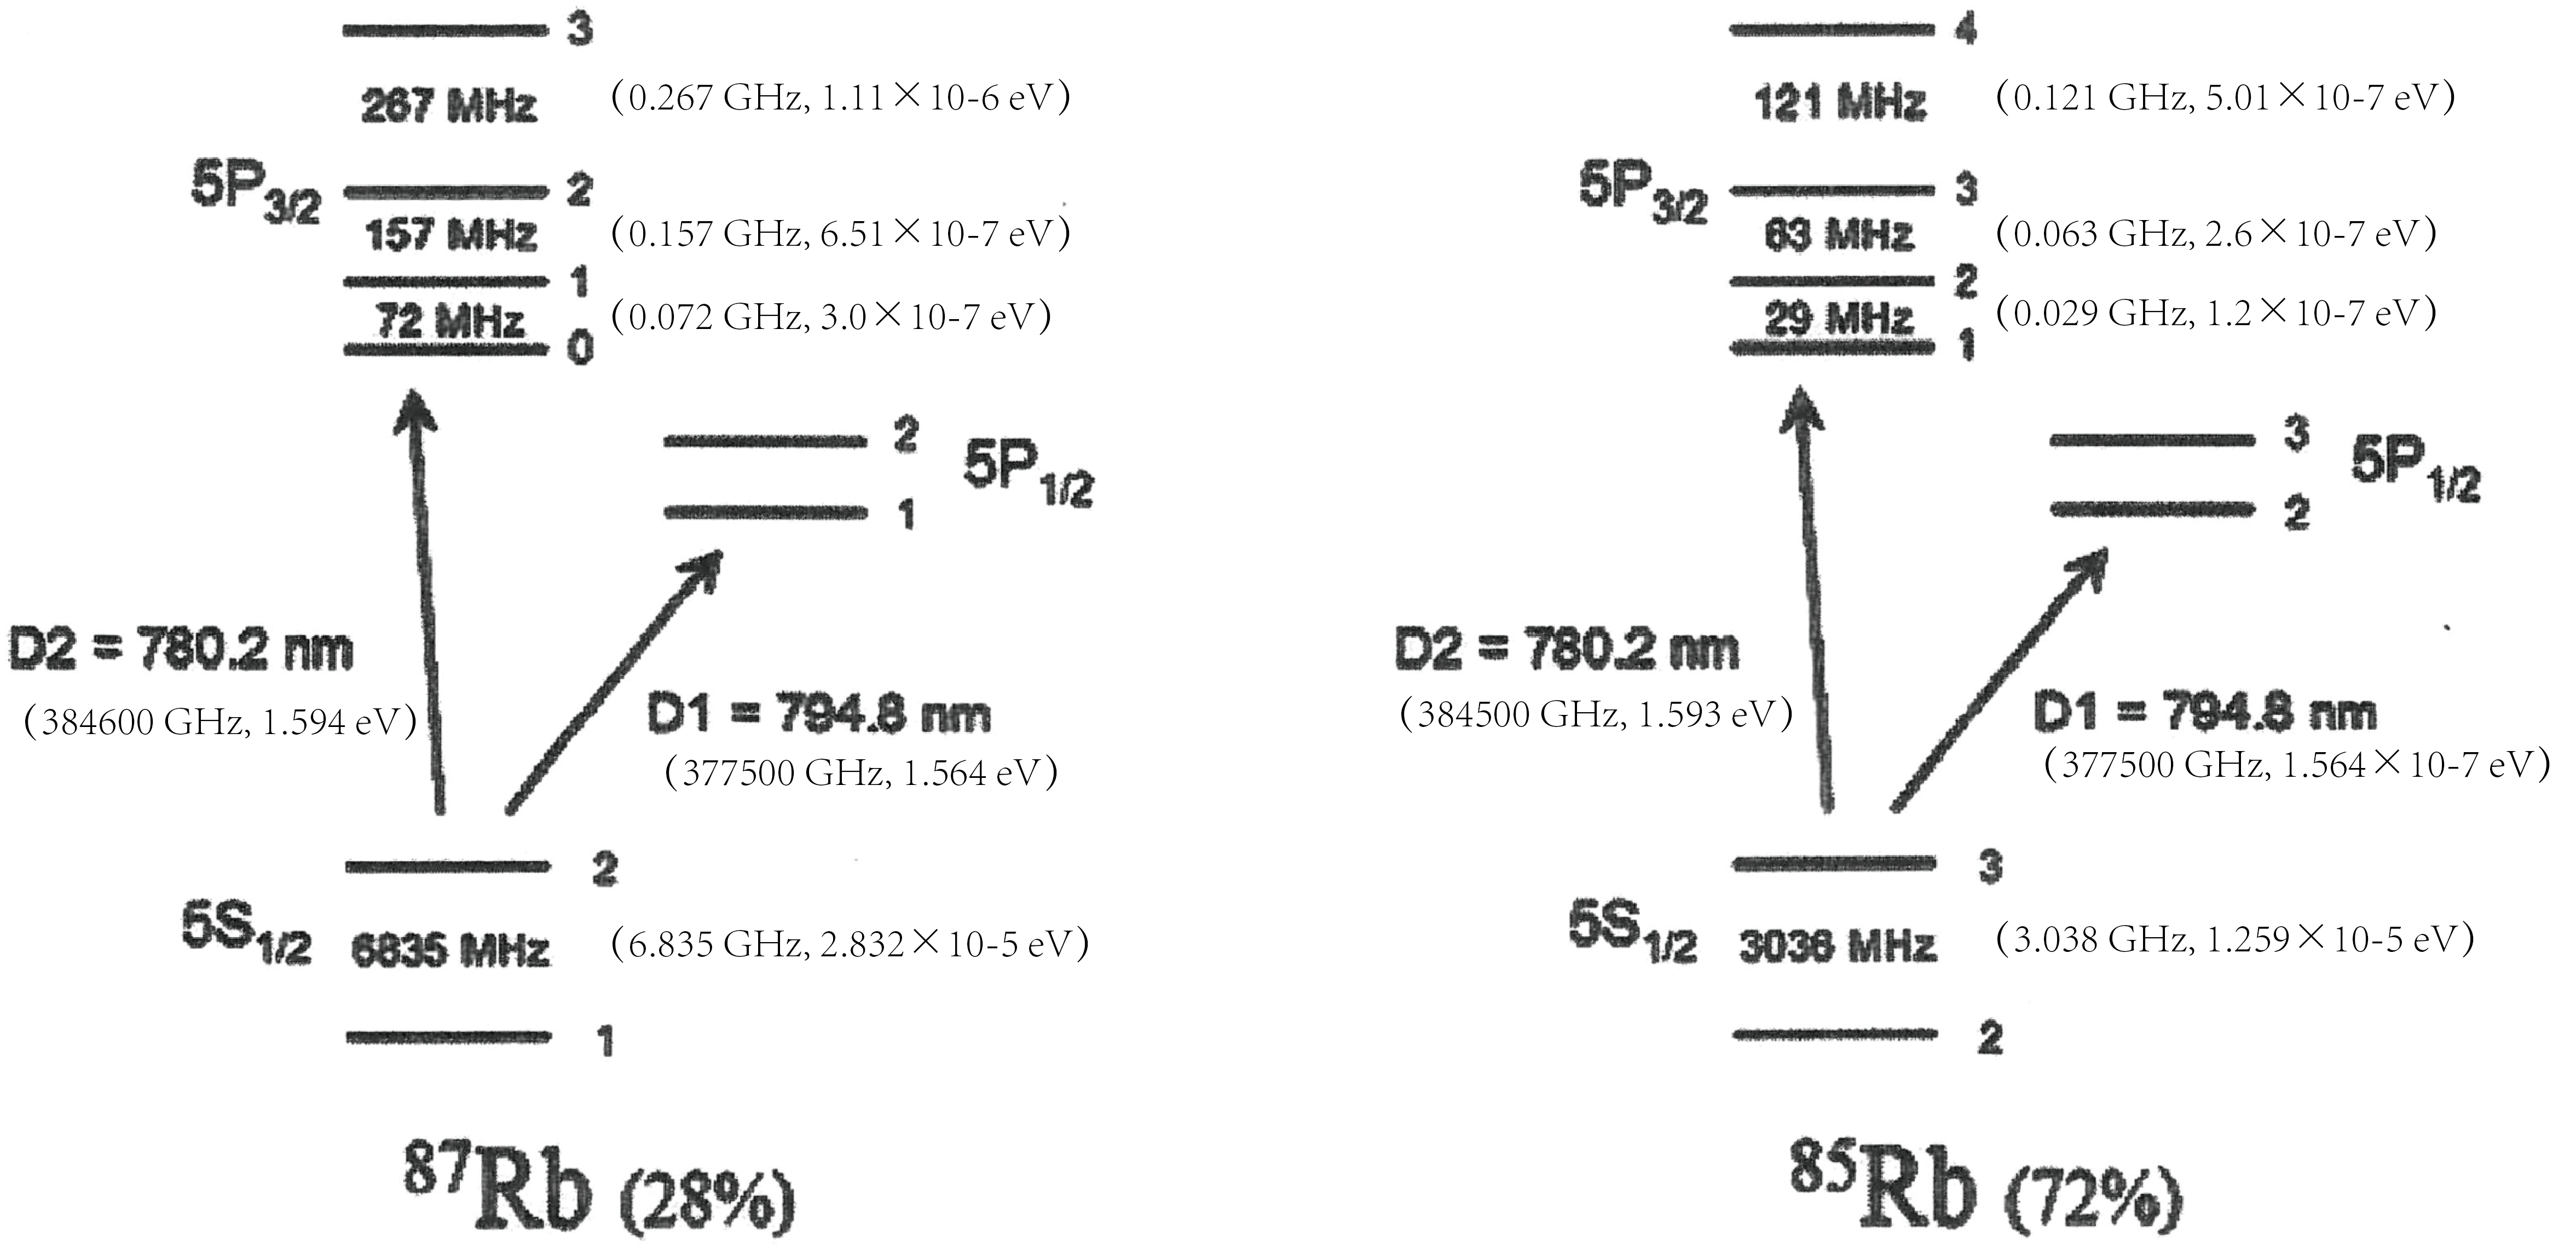
\includegraphics[width=.9\textwidth]{Rb-energy-level-1.png}
    \caption{铷原子能级结构(局部)}
    \label{Rb-energy-level}
\end{figure}

\section{铷原子谱线的多普勒展宽}
实验中测得的铷原子谱线并非分立的狄拉克函数状的特征峰,而是存在一定的展宽. 谱线的展宽主要由两种原因导致:
\begin{itemize}
    \item[(1)] 不确定原理和有限的能级寿命共同导致的洛伦兹展宽;
    \item[(2)] 热运动的原子的多普勒效应导致的多普勒展宽.
\end{itemize}
后者量级($10^{-6}e$V,具体计算见下文)远大于前者($10^{-11}\sim 10^{-8}e$V),做主要贡献. 下面我们分别从头推导气体中原子速度的麦克斯韦分布律和相对论多普勒效应,从而结合得到多普勒线型公式,并计算本实验场景下铷原子的光谱展宽.

\subsection{玻尔兹曼分布和麦克斯韦速度分布的证明}

\subsubsection{玻尔兹曼分布的证明}
首先,我们根据平衡态统计物理的基本假设——等概率原理推导玻尔兹曼分布.

玻尔兹曼系统是一个经典的(即非量子的)统计物理模型,其有如下两个基本设定:
\begin{itemize}
    \item[(1)] 各个粒子可分辨;
    \item[(2)] 每个量子态上可容纳的粒子数不受限制.
\end{itemize}

对于能级为$\epsilon_1,\epsilon_2,\cdots,\epsilon_l,\cdots$,各个能级的简并度分别为$\omega_1,\omega_2,\cdots,\omega_l,\cdots$,且各个能级上的粒子数分别为$a_1,a_2,\\\cdots,a_l,\cdots$,总粒子数为$\sum_la_l=N$的玻尔兹曼系统,要完全确定这一系统的状态,分为两步:
\begin{itemize}
    \item[(1)] 首先确定即占据能级$\epsilon_l$的,是哪$a_l$个粒子;
    \item[(2)] 其次确定各能级的微观状态,即能级$\epsilon_l$上的这$a_l$个粒子中的每个粒子分别在哪个量子态上(简并度为$\omega_l$,也就是说有$\omega_l$个量子态).
\end{itemize}
当分布($\{a_l\}$)给定,第一步就相当于把$N$个小球(粒子)放入容量分别为$a_1,a_2,\cdots,a_l,\cdots$的柜子(能级)中(具体在容器中如何排列先不管),一共有$\frac{N!}{\prod_la_l!}$中可能的情况. 而确定能级$\epsilon_l$上的微观状态,就相当于这$a_l$个小球中的每一个,都要选择占据$l$号柜子的$\omega_l$个抽屉(简并状态)哪一个,故能级$\epsilon_l$具有$\omega_l^{a_l}$个可能的微观状态. 考虑所有能级,有$\prod_l\omega_l^{a_l}$种可能的微观状态. 综合起来,当分布$\{a_l\}$给定,这一玻尔兹曼系统共有$\Omega=\frac{N!}{\prod_la_l!}\prod\omega_l^{a_l}$种可能的微观状态.

根据等概率原理,对于处在平衡态的孤立系统,每个可能的微观状态出现的概率相等. 因此系统的可能微观状态数最多的分布,就是系统最可能出现的分布,称最概然分布. 玻尔兹曼系统的最概然分布称玻尔兹曼分布. 利用变分原理可求出玻尔兹曼分布,对微观状态数取对数,
\begin{align}
    \ln\Omega=\ln N!-\sum_l\ln a_l!+\sum_l a_l\ln\omega_l,
\end{align}
在$\alpha_l$很大(那么$N$也很大)的情况下,利用斯特林公式有
\begin{align}
    \notag\ln\Omega\approx&N(\ln N-1)-\sum_la_l(\ln a_l-1)+\sum_l a_l\ln\omega_l\\
    =&N\ln N-\sum_l a_l\ln a_l+\sum_l a_l\ln\omega_l.
\end{align}
在最概然分布下,$\Omega$达到最大值,假设$a_l$有$\delta a_l$的微小变化,则$\ln\Omega$对应变化$\ln\Omega$应等于$0$,即
\begin{align}
    \delta\ln\Omega=-\sum_la_l\frac{1}{a_l}\delta a_l-\sum_l\ln a_l\delta a_l+\sum_l\ln\omega_l\delta a_l.
\end{align}
此外,由于$\delta a_l$不完全是独立的,而是满足
\begin{align}
    \label{N-const}\delta N=&\sum_l\delta a_l=0,\qquad(\text{孤立系统平衡状态下总粒子数不变})\\
    \label{E-const}\delta E=&\sum_l\epsilon_l\delta a_l=0,\qquad(\text{孤立系统平衡状态下总能量不变})
\end{align}
故有
\begin{align}
    \delta\ln\Omega=-\sum_l\ln\left(\frac{a_l}{\omega_l}\right)\delta a_l=0.
\end{align}
且由于这两个约束条件(式\eqref{N-const}\eqref{E-const}),需要引入两个拉格朗日未定乘子$\alpha$和$\beta$,
\begin{align}
    \delta\ln\Omega-\alpha\delta N-\beta\delta E=-\sum_l\left(\ln\frac{a_l}{\omega_l}+\alpha+\beta\epsilon_l\right)\delta\alpha_l=0,
\end{align}
根据拉氏乘子法原理,上述求和中每一项的系数都为零,
\begin{align}
    \ln\frac{a_l}{\omega_l}+\alpha+\beta\epsilon_l=0,
\end{align}
从而各能级上的粒子数为
\begin{align}
    a_l=\omega_le^{-\alpha-\beta\epsilon_l}.
\end{align}
能量为$\epsilon_l$的量子态上的粒子数为
\begin{align}
    f_l=e^{-\alpha-\beta\epsilon_l},
\end{align}
此即玻尔兹曼分布.

上面玻尔兹曼分布表达式中的常数$\alpha$和$\beta$可利用系统的各个物理量之间的关系来确定. 方便起见,我们定义配分函数
\begin{align}
    Z=\sum_l\omega_le^{-\beta\epsilon_l}.
\end{align}
将系统的各物理量用配分函数表示:粒子数为
\begin{align}
    N=\sum_la_l=\sum_l\omega_le^{-\alpha-\beta\epsilon_l}=e^{-\alpha}\sum_l\omega_le^{-\beta\epsilon_l}=e^{-\alpha}Z.
\end{align}
内能为
\begin{align}
    \notag U=&\sum_l\epsilon_la_l=\sum_l\epsilon_l\epsilon_le^{-\alpha-\beta\epsilon_l}=e^{-\alpha}\sum_l\omega_l\epsilon_le^{-\beta\epsilon_l}=e^{-\alpha}\left(-\frac{\partial}{\partial\beta}\sum_l\omega_le^{-\beta\epsilon_l}\right)=e^{-\alpha}\left(-\frac{\partial Z}{\partial\beta}\right)=\frac{N}{Z}\left(-\frac{\partial Z}{\partial\beta}\right)\\
    =&-N\frac{\partial}{\partial\beta}\ln Z.
\end{align}
广义力为
\begin{align}
    Y=\sum_l\frac{\partial\epsilon_l}{\partial y}a_l=\sum_l\frac{\partial\epsilon_l}{\partial y}\omega_le^{-\alpha-\beta\epsilon_l}=e^{-\alpha}\left(-\frac{1}{\beta}\frac{\partial}{\partial y}\right)\sum_l\omega_le^{-\beta\epsilon_l}=\frac{N}{Z}\left(-\frac{1}{\beta}\frac{\partial}{\partial y}\right)Z=-\frac{N}{\beta}\frac{\partial}{\partial y}\ln Z.
\end{align}
(特别地,当广义坐标$y$为体积$V$,广义力$Y$即为取负值的压强$-p$.)\\
一方面,根据热力学第一定律,我们有
\begin{align}
    dQ=dU-Y\,dy=dU-Y\,dy=-Nd\left(\frac{\partial}{\partial\beta}\ln Z\right)+\frac{N}{\beta}\frac{\partial\ln Z}{\partial y}dy.
\end{align}
上式两边同乘$\beta$有
\begin{align}
    \label{betadQ}
    \notag\beta dQ=&-N\beta d\left(\frac{\partial}{\partial\beta}\ln Z\right)+N\frac{\partial\ln Z}{\partial y}dy\\
    \notag&[\text{利用}d\left(N\beta\frac{\partial\ln Z}{\partial\beta}\right)=N\beta\,d\left(\frac{\partial\ln Z}{\partial\beta}\right)+N\frac{\partial\ln Z}{\partial\beta}d\beta]\\
    \notag=&-\left[d\left(N\beta\frac{\partial\ln Z}{\partial\beta}\right)-N\frac{\partial\ln Z}{\partial\beta}d\beta\right]+N\frac{\partial\ln Z}{\partial y}dy\\
    \notag=&-d\left(N\beta\frac{\partial\ln Z}{\partial\beta}\right)+d\left(N\ln Z\right)\\
    =&d\left(N\ln Z-N\beta\frac{\partial\ln Z}{\partial\beta}\right).
\end{align}
另一方面,根据热力学基本方程,
\begin{align}
    \label{dQ/T}
    \frac{dQ}{T}=\frac{dU-Y\,dy}{T}=dS.
\end{align}
对比式\eqref{betadQ}和\eqref{dQ/T},我们可以推断$\beta$和$\frac{1}{T}$都是积分因子,两者应该相差一个常数,即
\begin{align}
    \beta=\frac{1}{k_BT}.
\end{align}
其中的常数$k_B$称为玻尔兹曼常数,如果我们将上面计算各个物理量的式子运用到理想气体,我们就可以得到
\begin{align}
    k_B=1.38\times 10^{-23}\text{J}\cdot\text{K}^{-1}.
\end{align}

对于稀薄的铷原子蒸汽,由于各气体粒子(原子或分子)之间间隔很大,相互作用很微弱,从而可认为各气体粒子可分辨,且每个量子态上可容纳的(即具有相同平动速度的)粒子数量不受限制,因此铷原子蒸汽符合玻尔兹曼系统的设定,从而遵循玻尔兹曼分布.

\subsubsection{麦克斯韦速度分布律的证明}
将玻尔兹曼分布应用于只有平动动能的气体粒子,可以证明麦克斯韦速度分布律.

设气体含有$N$个粒子,体积为$V$. 每个粒子的平动动能为
\begin{align}
    \epsilon=\frac{1}{2m}(p_x^2+p_y^2+p_z^2).
\end{align}
无论是用经典的方法(周期性边界条件),还是用量子的方法(不确定性原理),我们都可以推出,相空间(以粒子的广义坐标和广义动量为坐标构成的空间)的单位体积内都只能容纳有限个数的状态. 假设平均每个平动状态所占据相空间中的体积为$h_0^3$,则体积$V$,动量范围$dp_xdp_ydp_z$对应的相空间中,所能容纳的平动状态数为
\begin{align}
    \frac{V}{h_0^3}dp_x\,dp_y\,dp_z.
\end{align}
(这里的状态数实际上和上一小小节中的能级的简并度$\omega_l$是同一个东西.)\\
因此能量为$\epsilon$的粒子数为
\begin{align}
    a=\frac{V}{h_0}e^{-\alpha-\beta\epsilon}dp_x\,dp_y\,dp_z.
\end{align}
(因为对于经典粒子,物理量是连续的,所以这里略去了下标$l$.)\\
由于总分子数为
\begin{align}
    \notag N=&\frac{V}{h_0^3}\int_{-\infty}^{+\infty}\int_{-\infty}^{+\infty}\int_{-\infty}^{+\infty}e^{-\alpha-\frac{\beta}{2m}\left(p_x^2+p_y^2+p_z^2\right)}\,dp_x\,dp_y\,dp_z\\
    \notag=&\frac{V}{h_0^3}e^{-\alpha}\left(\int_{-\infty}^{+\infty}e^{-\frac{\beta}{2m}p_x^2}\,dp_x\right)^3\\
    \notag&[\text{利用}\int_0^{+\infty}e^{-\alpha x^2}\,dx=\frac{1}{2}\sqrt{\frac{\pi}{\alpha}}]\\
    =&\frac{V}{h_0^3}\frac{1}{8}\left(\frac{2m\pi}{\beta}\right)^{3/2}
\end{align}
得到系数
\begin{align}
    e^{-\alpha}=\frac{N}{V}\left(\frac{h_0^2}{2\pi mkT}\right)^{3/2}.
\end{align}
故质心动量在$dp_x\,dp_y\,dp_z$范围内的粒子数为
\begin{align}
    a=N\left(\frac{1}{2\pi mk_BT}\right)^{3/2}e^{-\frac{1}{2k_BmT}\left(p_x^2+p_y^2+p_z^2\right)}\,dp_x\,dp_y\,dp_z.
\end{align}
用速度作为变量代换动量,即$p_x=mv_x$,$p_y=mv_y$,$p_z=mv_z$,有
\begin{align}
    a=N\left(\frac{m}{2\pi k_BT}\right)^{3/2}e^{-\frac{m}{2k_BT}\left(v_x^2+v_y^2+v_z^2\right)}\,dv_x\,dv_y\,dv_z.
\end{align}
这就得到了麦克斯韦速度分布律,它描述了单位体积内,速度在$dv_x\,dv_y\,dv_z$范围内的粒子数:
\begin{align}
    dn(v_x,v_y,v_z)=\frac{N}{V}\left(\frac{m}{2\pi k_BT}\right)^{3/2}e^{-\frac{m}{2k_BT}\left(v_x^2+v_y^2+v_z^2\right)}\,dv_x\,dv_y\,dv_z.
\end{align}

\subsubsection{相对论性多普勒效应的证明}
假设真空中的观察者(用字母o表示)与波源(用字母s表示)以一相对速度$v$彼此远离. 以波源为参考系,两个相邻波峰的距离为
\begin{align}
    \lambda=\frac{c}{\nu_c},
\end{align}
其中$c$为光速,$f_s$为波源发出的光波的原始频率. 观察者接受到两个相邻波峰的时间间隔为
\begin{align}
    t=\frac{\lambda}{c-v}=\frac{1}{(1-v/c)\nu_s}.
\end{align}
在观察者的参考系找那个,对于观察者来说,他所认为的接受到两个相邻波峰的时间间隔为
\begin{align}
    t_o=\sqrt{1-\frac{v^2}{c^2}}t=\sqrt{\frac{1+v/c}{1-v/c}}t_o,
\end{align}
所以观察者探测到的光波的频率为
\begin{align}
    \nu_o=\sqrt{\frac{1-v/c}{1+v/c}}\nu_s.
\end{align}
若处于折射率为$\mu$的介质中,上式变为
\begin{align}
    \nu_o=\sqrt{\frac{1-\mu v/c}{1+\mu v/c}}\nu_s.
\end{align}
更一般地,当观察者以速度$v$沿着与两者连线夹角为$\theta$(在波源参考系中观察到的角度)的方向远离波源,则表达式为
\begin{align}
    \nu_o=\frac{1-\frac{v\cos\theta}{c}}{\sqrt{1-v^2/c^2}}\nu_s.
\end{align}

\subsubsection{多普勒展宽的推导}
结合麦克斯韦速度分布律和多普勒效应,我们就可以推导出多普勒展宽.\\

由上一小小节的结论可以看出,横向多普勒效应远小于纵向多普勒效应,故只需考虑沿着激光传输方向的速度分布及其造成的多普勒效应,铷蒸汽中原子运动速度远小于光速,在低速下频率公式可取一阶近似,有
\begin{align}
    \label{Doppler}
    \nu=\left(1+\frac{v_z}{c}\right)\nu_0,
\end{align}
其中$\nu_0$为铷原子的能级跃迁频率,$\nu$为实际吸收激光的频率. 沿激光传输方向速度分量在$v_z\sim v_z+dv_z$范围内原子占总数的比例为
\begin{align}
    \frac{dn_z}{n_z}=\left(\frac{m}{2\pi k_BT}\right)^{1/2}e^{-\frac{mv_z^2}{2k_BT}}\,dv_z
\end{align}
利用式\eqref{Doppler},用吸收频率作为变量代换速度,可以得到在$\nu\sim\nu+d\nu$范围内的光强在总光强中的占比
\begin{align}
    f_D(\nu)=\frac{dn_z/n}{d\nu}=\left(\frac{m}{2\pi k_BT}\right)^{1/2}\exp\left[-\frac{mc^2(\nu-\nu_0)^2}{2kT\nu_0^2}\right]\frac{c}{\nu_0}.
\end{align}
解方程
\begin{align}
    f_D\left(\nu_0-\frac{\Delta\nu}{2}\right)=f_D\left(\nu_0+\frac{\Delta\nu}{2}\right)=\frac{1}{2}f_D(\nu_0)
\end{align}
得到多普勒展宽
\begin{align}
    \Delta\nu=2\nu_0\left(\frac{2k_BT}{mc^2}\ln 2\right)^{1/2}.
\end{align}

\subsection{计算}
代入铷原子的质量$m=\frac{85.5\times 10^{-3}\text{kg}\cdot\text{mol}^{-1}}{6.02\times 10^{23}\text{mol}^{-1}}=1.42\times 10^{-25}$kg,P$_{3/2}$到S$_{1/2}$的跃迁频率$\nu_0=384600$GHz,温度$T=50^{\circ}\text{C}=323$K,铷原子蒸汽的多普勒展宽为
\begin{align}
    \Delta\nu=2\nu_0\left(\frac{2k_BT}{mc^2}\ln 2\right)^{1/2}=0.535\text{GHz},\qquad(2.22\times 10^{-6}e\text{V}).
\end{align}

\section{讨论}
前两节的计算结果表明,铷原子蒸汽光谱的多普勒展宽量级远大于P$_{3/2}$超精细结构的劈裂,因此根据瑞利判据,单纯利用吸收光谱是无法分辨出超精细结构的.

\end{document}